% $$L_{cyc}^k=L_{CE}(A_t^{t+k}A_{t+k}^t, I)$$
\subsection{Normal-assisted Random Walk}

% \begin{figure*}
%     \centering
%     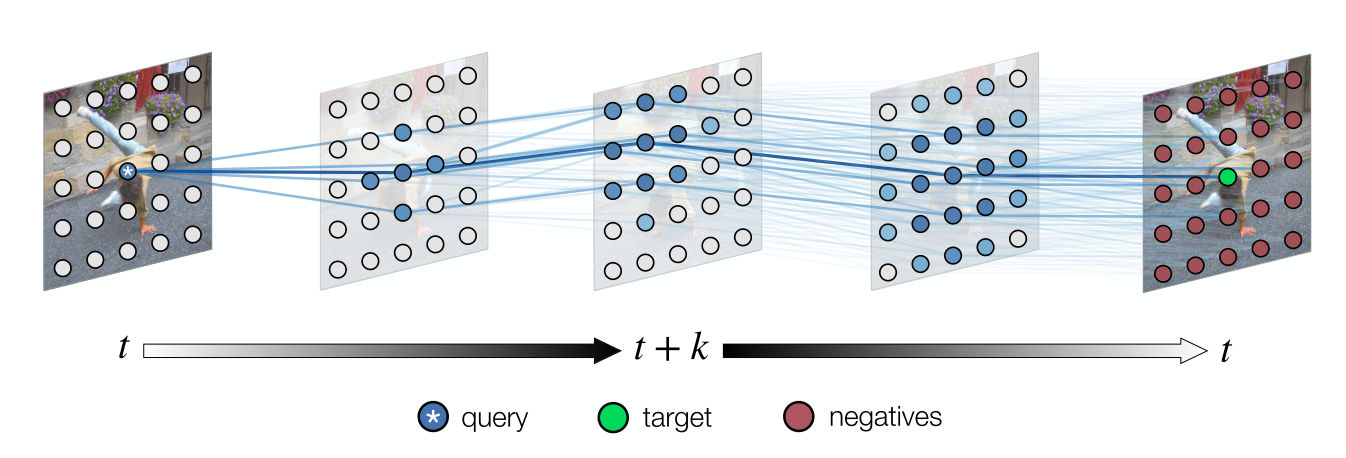
\includegraphics[width=1.0\linewidth]{FinalReport/random_walk.png}
%     \caption{Figure credit \cite{jabri2020walk}. Following there approach, we represent video as a graph, where nodes are image patches, and edges are product of 2D affinities (in some feature space) and 3D distance of detected normal vectors between nodes of neighboring frames.  Our aim is to learn features such that temporal correspondences are represented by strong edges we learn to find paths through the graph by performing a random walk between query and target nodes.  A contrastive loss with affinities times the  encourages paths that reach the target, implicitly supervising latent correspondence along the path. Learning proceeds without labels by training on a palindrome sequence, walking from frame t to t+k, then back to t, using the initial node itself as the target}
%     \label{fig:random_walk}
% \end{figure*}
\begin{figure*}
    \centering
    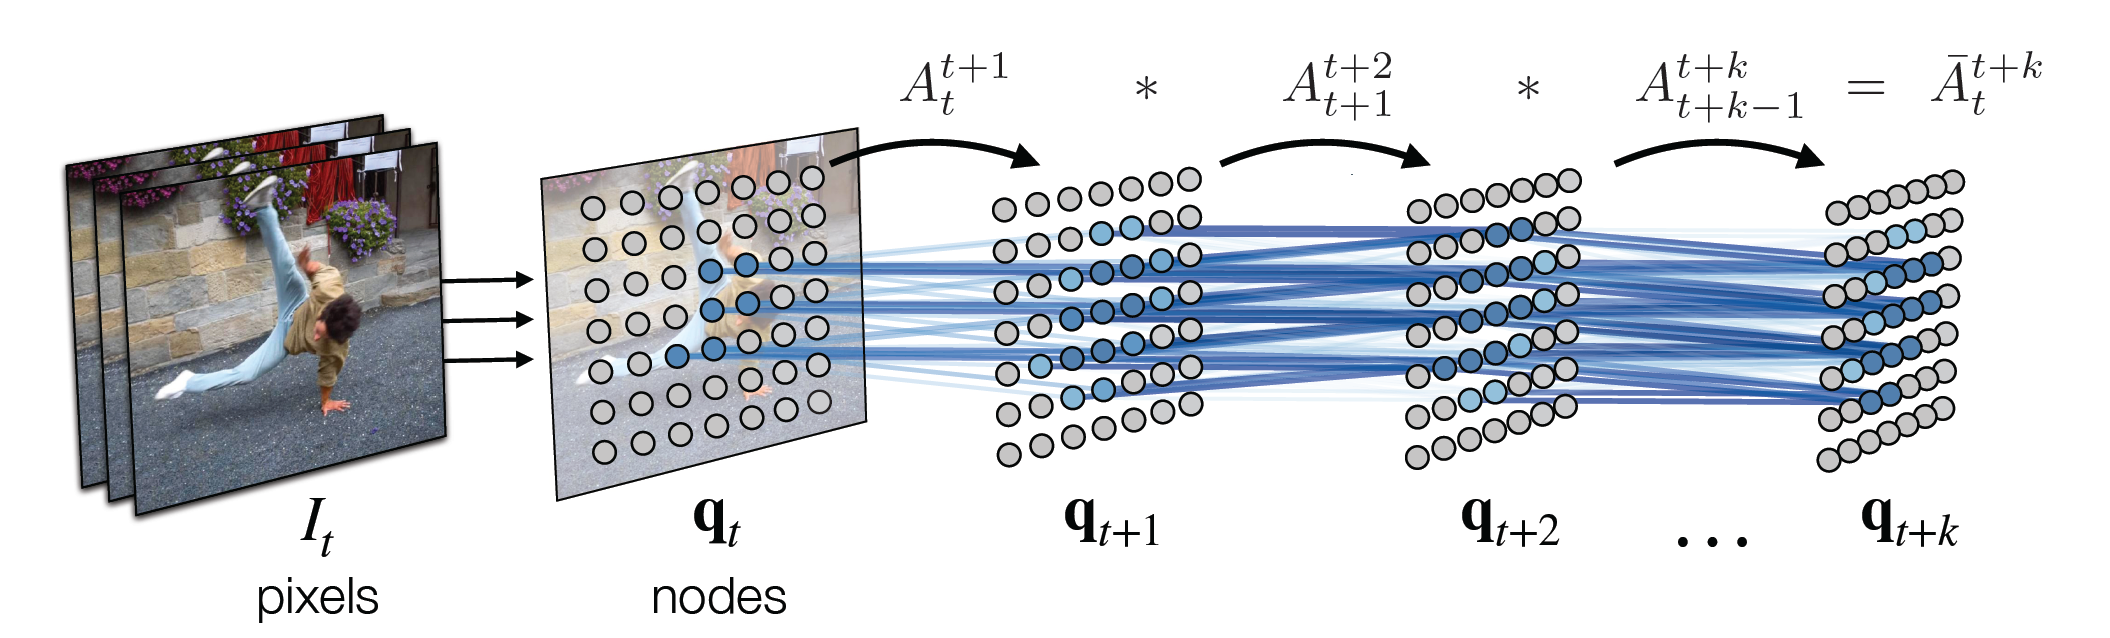
\includegraphics[width=0.8\linewidth]{FinalReport/markov.png}
    \vspace{-0.1in}
    \caption{Figure credit \cite{jabri2020walk}. \textbf{Correspondence as a Random Walk.} We build a space-time graph by extracting nodes from each frame and allowing directed edges between nodes in neighboring frames. The transition probabilities of a random walk along this graph are determined by the product of 2D pairwise similarity in a learned representation and 3D distance of normal vectors detected by a PlaneRCNN network.
    }
    \vspace{-0.1in}
    \label{fig:markov}
\end{figure*}
 \begin{figure*}
    \centering
    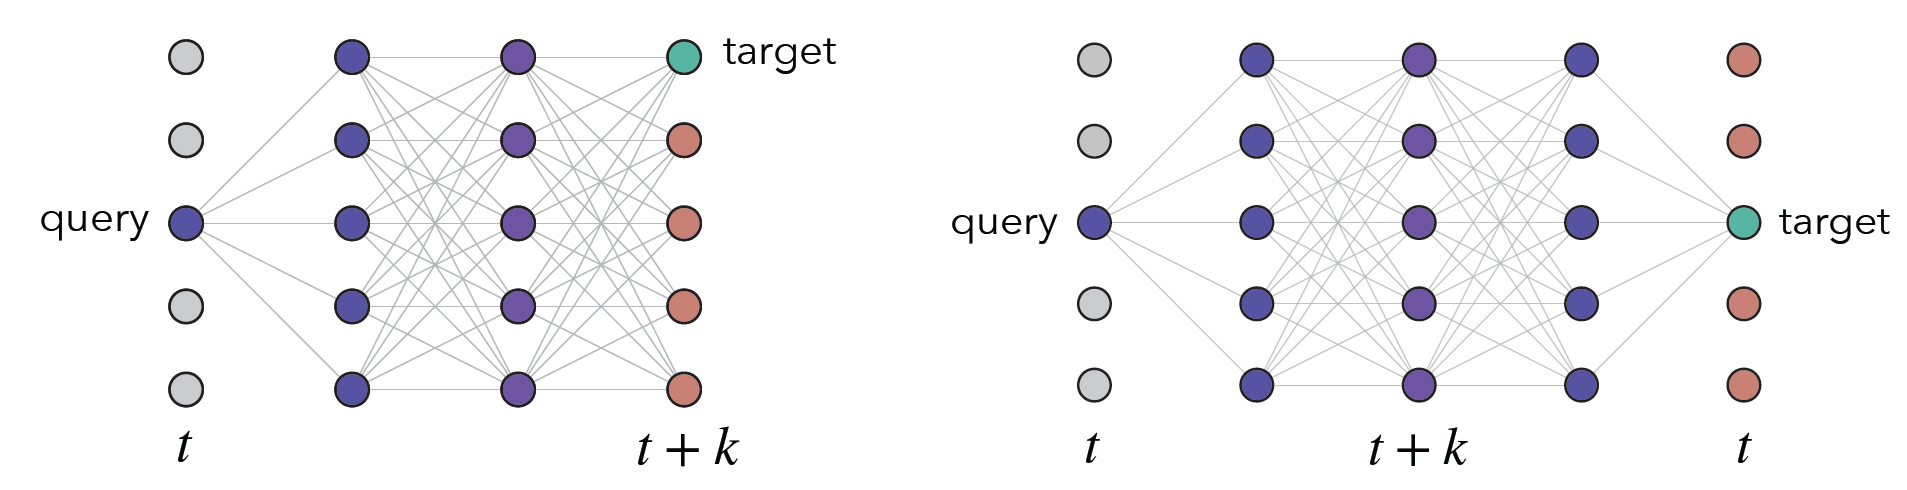
\includegraphics[width=0.8\linewidth]{FinalReport/palindrome.png}
    \vspace{-0.1in}
    \caption{Figure credit \cite{jabri2020walk}. \textbf{Guiding the walk with palindrome self-supervision.} (a) Specifying a target multiple steps in the future provides implicit supervision for latent correspondences along each path (\textit{left}). (b) We can construct targets for free by choosing palindromes as sequences for learning (\textit{right}).
    }
        \vspace{-0.15in}
    \label{fig:palindrome}
\end{figure*}
\vspace{-0.1in}
Following~\cite{jabri2020walk}, we represent each video as a directed graphs with nodes being patches of each frame and edges connect nodes in neighboring frames. Let $\mathbf{I}$ be a set of frames from a video and $\mathbf{q}_{t}$ be the set of $N$ nodes extract from frame $I_{t}$. We train an encoder $\phi$ which maps nodes to $l_2$-normalized $d-$dimensional vectors, which we use to compute a pairwise 2D similarity function between nodes $d_{\phi}(q_{1}, q_{2}) = \langle \phi(q_{1}),\phi(q_{2}) \rangle$ and an 2D embedding matrix for $\mathbf{q}_{t}$ denoted $Q_{t} \in \mathbb{R}^{N\times d}$. We convert pairwise similarities into non-negative affinities by applying a softmax (with temperature $\tau = 0.07$) over edges departing from each node. For timesteps $t$ and $t+1$, the stochastic matrix of 2D affinities is 
\vspace{-0.1in}
\begin{equation}
\small
    A_t^{t+1}(i,j) = \texttt{softmax}(Q_{t},Q^{\text{T}}_{t+1})_{ij} = \frac{\exp(d_{\phi}(\mathbf{q}_{t}^{i}, \mathbf{q}_{t+1}^{j})/\tau)}{\sum_{l=1}^{N}d_{\phi}(\mathbf{q}_{t}^{i}, \mathbf{q}_{t+1}^{l})/\tau)}
\end{equation}



Our modification applies here that we add 3D normal vector distance (normal vector prediction process are detailed in Section \ref{normal}) aside from the 2D embedding affinities to the stochastic matrix.  Let $\mathbf{n}_{t}$ be the set of $N$ normal vector extracted from frame $\mathbf{I}_{t}$, we construct our modified stochastic matrix by multiplying the raw 2D affinity probability $A_t^{t+1}(i,j)$ with the 3D normal eculidean distance $||\mathbf{n}_{t}^{i}-\mathbf{n}_{t+1}^{j}||^2$, and we further apply a softmax to obtain a probability. For timesteps $t$ and $t+1$, our modified stochastic matrix is

\vspace{-0.15in}

\begin{equation}\small
    A_t^{t+1}'(i,j) =  \frac{\exp(A_t^{t+1}(i,j)\cdot ||\mathbf{n}_{t}^{i}-\mathbf{n}_{t+1}^{j}||^2)}{\sum_{l=1}^{N}\exp(A_t^{t+1}(i,j)\cdot ||\mathbf{n}_{t}^{i}-\mathbf{n}_{t+1}^{l}||^2)}
\end{equation}

Note that this describes only the local affinity between the patches of two video frames, $\mathbf{q}_{t}$ and $\mathbf{q}_{t+1}$, and we relate all nodes in the video as a Markov chain following~\cite{jabri2020walk}. Given the spatio-temporal connectivity of the graph, a step of a random walker on this graph can be viewed as performing tracking by \textit{contrasting} similarity of neighboring nodes. Let $X_{t} $ be the state of the walker at time $t$, with transition probabilities $A_t^{t+1}'(i,j) = P(X_{t+1}=j | X_{t} = i)$, where $P(X_t =i)$ is the probability of being at node $i$ at time $t$. And we can formulate long-range correspondence as walking multiple steps along the graph (Figure \ref{fig:markov}):
\vspace{-0.1in}
\begin{equation}\small
A^{t+k}_{t} = P(X_{t+k}|X_{t}) = \prod^{k-1}_{i=0}A_{t+i}^{t+i+1}
\end{equation}
\vspace{-0.1in}
 
 \par \noindent {\bf Guiding the walk with palindrome self-supervision.}
 Our aim is to train the encoder $\phi$ to encourage the random walker to follow paths of corresponding patches as it steps through time. Following~\cite{jabri2020walk}, we train our model with a cross-entrophy loss on the \textit{palindrome} self-supervised training examples. To formalize, given a sequence of frames ($I_t, \dots, I_{t+k}$), we form training examples by simply concatenating the sequence with a temporally reversed version of itself: ($I_t, \dots, I_{t+k}, \dots, I_{t}$). Treating each query node's position as its own target (as shown in Figure \ref{fig:palindrome}), we obtain the following cycle-consistency cross-entropy objective which maximize the likelihood that a walker beginning at a query node at $t$ ends at the same target node at time $t + 2k$:
 \vspace{-0.1in}
\begin{equation}\small
 \mathcal{L}
^{k}_{cyc} = \mathcal{L}_{CE}(A^{t+k}_{t}A^{t}_{t+k}, I) = - \sum_{i=1}^{N} \log P(X_{t+2k}=i|X_{t} = i)
\end{equation}
 
As the model computes a soft attention distribution at every time step, we can backpropagate loss across – and thus learn from – the many alternate paths of similarity that link query and target nodes.
 
\par \noindent {\bf Pixel to nodes.\label{pix}}
We sample $64 \times 64$ patches on a $640\times 480$ image with stride of $32$ to allow overlapping. Following \cite{jabri2020walk} and \cite{long2015fully}, we reuse the convolutional feature map between patches obtained from training for testing instead of processing the patches independently and thus features could be extracted with only a single feed-forward pass.

 \par \noindent {\bf Encoder $\phi$. \label{encoder}}
We use ResNet-18 \cite{he2016deep} for the encoder which outputs a 128-dimensional vector for each patch. We apply a linear projection and $l_2$ normalization after the last average pooling layer and modifies the last 2 \texttt{res3} and \texttt{res4} layer to have stride of 1 instead of 2 following \cite{jabri2020walk}.

% \begin{equation}
%     A_t^{t+1}(i,j) \leftarrow P(X_{t+1}=j|X_t=i)\times||n_i-n_j||^2    
%     \label{eqn:normal-assist}
% \end{equation}


\subsection{Normal Prediction for Patches \label{normal}}
\par \noindent {\bf Plane detection.} We follow PlaneRCNN~\cite{liu2019planercnn} to detect planes in each frame. Instead of using the whole pipeline for prediction, we only use the plane detection network in~\cite{liu2019planercnn} and ignore the segmentation refinement network and warping loss module for simplicity. 
The plane detection network uses ResNet50-FPN~\cite{lin2017feature} as the backbone.
A region proposal network is used to extract box proposals. The plane masks and normals are inferred from features from RoIAlign~\cite{he2017mask}. The PlaneRCNN is supervised by ground truth label on ScanNet generated by fitting planes on the original house mesh provided by~\cite{liu2018planenet}. 
\par \noindent {\bf Patch normal assignment.} For each patch, we calculate the GIoU \cite{Rezatofighi_2018_CVPR} between that patch and each bounding box of the plane masks and assign the normal vector of the mask with the highest GIoU. % GIoU is calculated using the following algorithm:



\subsection{Training Details}
Our Normal-assisted Random Walk network is trained on the Scannet training set, using one Tesla V100 GPU on Colab with learning rate 0.0001, batch size 4 and Adam optimizer with default parameters. The model is trained for 25 epochs. 

Our PlaneRCNN network is implemented in Detectron2 and is trained on the Scannet training set, using 2 GPUs with learning rate 0.001, batch size 16, and SGD optimizer with momentum 0.9. The model is trained for 80k iterations.
